%%% %%%%%%%%%%%%%%%%%%%%%%%%%%%%%%%%%%%%%%%%%%%%%%%%%%%%%%%%%%%%%%%%%%%%%%%%%%%%

\section{Human-Like Cognitive Architectures}

%%% %%%%%%%%%%%%%%%%%%%%%%%%%%%%%%%%%%%%%%%%%%%%%%%%%%%%%%%%%%%%%%%%%%%%%%%%%%%%

Our objective in developing systems that incorporate characteristics of human intelligence is three fold: First, humans provide a compelling solution to the problem of building intelligent systems that we can use as a basic blueprint and then improve upon. Second, the resulting AI systems are likely to be well suited to developing assistants that complement and extend human intelligence while operating in a manner comprehensible to human understanding. Finally, cognitive and systems neuroscience provide clues to engineers interested in exploiting what we know concerning how humans think about and solve problems. In this appendix, we demonstrate one attempt to concretely realize what we've learned from these disciplines in an architecture constructed from off-the-shelf neural networks. 

The programmer's apprentice relies on multiple sources of input, including dialogue in the form of text utterances, visual information from an editor buffer shared by the programmer and apprentice and information from a specially instrumented integrated development environment designed for analyzing, writing and debugging code adapted to interface seamlessly with the apprentice. This input is processed by a collection of neural networks modeled after the primary sensory areas in the primate brain. The output of these networks feeds into a hierarchy of additional networks corresponding to uni-modal secondary and multi-modal association areas that produce increasingly abstract representations as one ascends the hierarchy \emdash{} see Figure~{\urlh{#fig_Posterior_Cortex_Semantic_Memory}{50}}.
  
%%% %%%%%%%%%%%%%%%%%%%%%%%%%%%%%%%%%%%%%%%%%%%%%%%%%%%%%%%%%%%%%%%%%%%%%%%%%%%% 

\setcounter{figure}{49}

%%% %%%%%%%%%%%%%%%%%%%%%%%%%%%%%%%%%%%%%%%%%%%%%%%%%%%%%%%%%%%%%%%%%%%%%%%%%%%%

%%% Figure~{\urlh{#fig_Posterior_Cortex_Semantic_Memory}{50}}
\rawhtml
<a name="fig_Posterior_Cortex_Semantic_Memory"></a>
\endrawhtml
\begin{figure}
%
  \hrule{}
%
  \begin{center} 
    % (* 1.375 (/ 1106 2.00)) = 550 
    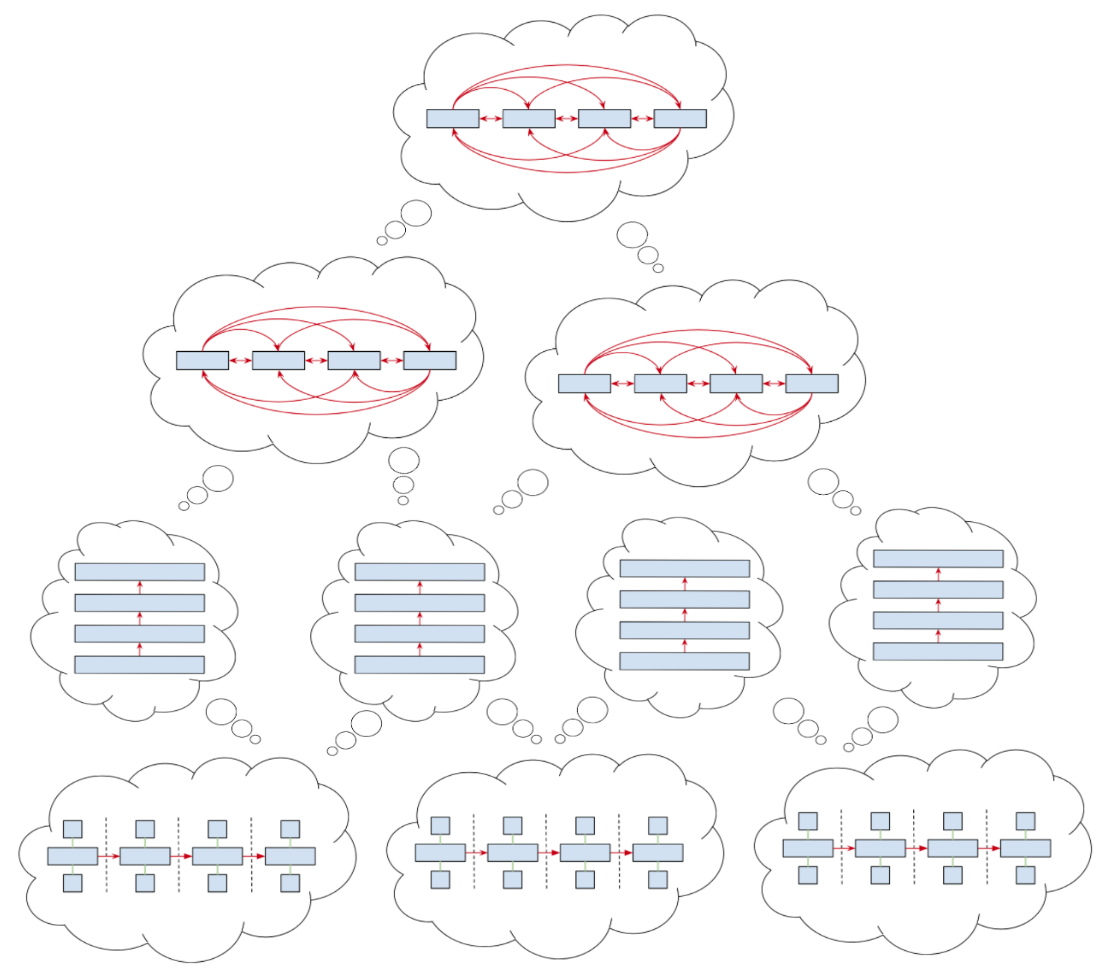
\includegraphics[width=550pt]{./figures/Posterior_Cortex_Semantic_Memory.png} % 1106 × 973 pixels
  \end{center}
%
  \caption{The architecture of the apprentice sensory cortex including the layers corresponding to abstract, multi-modal representations handled by the association areas can be realized as a multi-layer hierarchical neural network model consisting of standard neural network components whose local architecture is primarily determined by the sensory modality involved. This graphic depicts these components as encapsulated in thought bubbles of the sort often employed in cartoons to indicate what some cartoon character is thinking. Analogously, the technical term "thought vector" is used to refer to the activation state of the output layer of such a component.}
%
  \hrule{}
%
\end{figure}

%%% %%%%%%%%%%%%%%%%%%%%%%%%%%%%%%%%%%%%%%%%%%%%%%%%%%%%%%%%%%%%%%%%%%%%%%%%%%%%

Stanislas Dehaene and his colleagues at the Coll\`{e}ge de France in Paris developed a computational model of consciousness that provides a practical framework for thinking about consciousness that is sufficiently detailed for much of what an engineer might care about in designing digital assistants~\cite{Dehaene2014}. Dehaene’s work extends the {\it{Global Workspace}} Theory of Bernard Baars~\cite{Baars1988}. Dehaene’s version of the theory combined with Yoshua Bengio’s concept of a {\it{consciousness prior}} and deep reinforcement learning~\cite{MnihetalCoRR-13,NairetalCoRR-15} suggest a model for constructing and maintaining the cognitive states that arise and persist during complex problem solving~\cite{BengioCoRR-17}.

Global Workspace Theory accounts for both conscious and unconscious thought with the primary distinction for our purpose being that the former has been selected for attention and the latter has not been so selected. Sensory data arrives at the periphery of the organism. The data is initially processed in the primary sensory areas located in posterior cortex, propagates forward and is further processed in increasingly-abstract multi-modal association areas. Even as information flows forward toward the front of the brain, the results of abstract computations performed in the association areas are fed back toward the primary sensory cortex. This basic pattern of activity is common in all mammals. 

The human brain has evolved to handle language. In particular, humans have a large frontal cortex that includes machinery responsible for conscious awareness and that depends on an extensive network of specialized neurons called spindle cells that span a large portion of the posterior cortex allowing circuits in the frontal cortex to sense relevant activity throughout this area and then manage this activity by creating and maintaining the persistent state vectors that are necessary when inventing extended naratives or working on complex problems that require juggling many component concepts at once. Figure~{\urlh{#fig_Global_Workspace_Conscious_Attention}{51}} suggests a neural architecture combining the idea of a global workspace with that of an attentional system for identifying relevant input.

%%% %%%%%%%%%%%%%%%%%%%%%%%%%%%%%%%%%%%%%%%%%%%%%%%%%%%%%%%%%%%%%%%%%%%%%%%%%%%% 

\setcounter{figure}{50}

%%% %%%%%%%%%%%%%%%%%%%%%%%%%%%%%%%%%%%%%%%%%%%%%%%%%%%%%%%%%%%%%%%%%%%%%%%%%%%%

%%% Figure~{\urlh{#fig_Global_Workspace_Conscious_Attention}{51}}
\rawhtml
<a name="fig_Global_Workspace_Conscious_Attention"></a>
\endrawhtml
\begin{figure}
%
  \hrule{}
%
  \begin{center} 
    % (* 1.375 (/ 1063 2.00)) = 530
    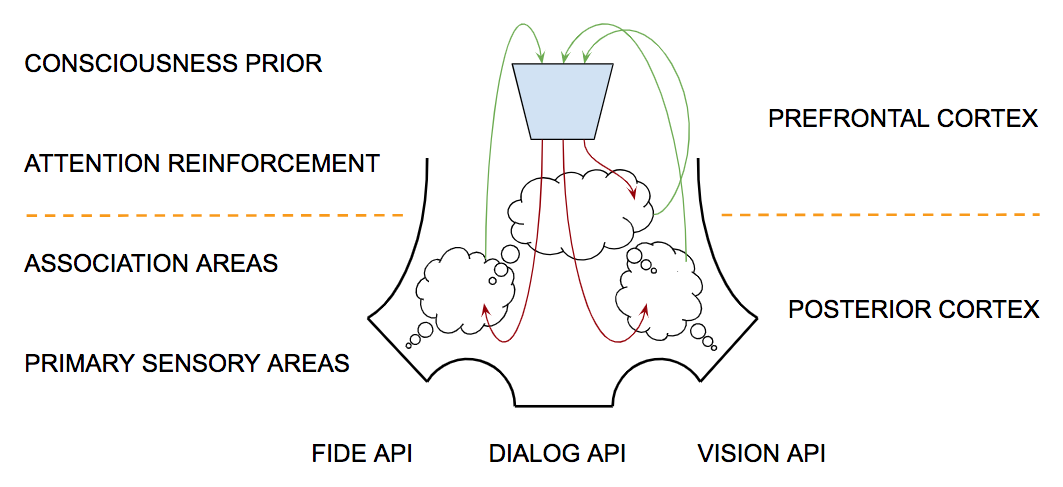
\includegraphics[width=530pt]{./figures/Global_Workspace_Conscious_Attention.png} % 1063 × 487 pixels
  \end{center}
%
  \caption{The basic capabilities required to support conscious awareness can be realized in a relatively simple computational architecture that represents the apprentice’s global workspace and incorporates a model of attention that surveys activity throughout somatosensory and motor cortex, identifies the activity relevant to the current focus of attention and then maintains this state of activity so that it can readily be utilized in problem solving.  In the case of the apprentice, new information is ingested into the model at the system interface, including dialog in the form of text, visual information in the form of editor screen images, and a collection of programming-related signals originating from a suite of software development tools. 
%
Single-modality sensory information feeds into multi-modal association areas to create rich abstract representations. Attentional networks in the prefrontal cortex take as input activations occurring throughout the posterior cortex. These networks are trained by reinforcement learning to identify areas of activity worth attending to and the learned policy selects a set of these areas to attend to and sustain. This attentional process is guided by a prior that prefers low-dimensional thought vectors corresponding to statements about the world that are either true, highly probable or very useful for making decisions. Humans can sustain only a few such activations at a time. The apprentice need not be so constrained.}
%
  \hrule{}
%
\end{figure}

%%% %%%%%%%%%%%%%%%%%%%%%%%%%%%%%%%%%%%%%%%%%%%%%%%%%%%%%%%%%%%%%%%%%%%%%%%%%%%%

Fundamental to our understanding of human cognition is the essential tradeoff between fast, highly-parallel, context-sensitive, distributed connectionist-style computations and slow, serial, systematic, combinatorial symbolic computations. In developing the programmer's apprentice, symbolic computations of the sort common in conventional computing are realized using extensions that provide a differentiable interface to conventional memory and information processing hardware and software. Such interfaces include the Neural Turing Machine~\cite{GravesetalCoRR-14} (NTM), Memory Network Model~\cite{WestonetalCoRR-14,SukhbaataretalCoRR-15} and Differentiable Neural Computer~\cite{GravesetalNATURE-16} (DNC).

The global workspace summarizes recent experience in terms of sensory input, its integration, abstraction and inferred relevance to the context in which the underlying information was acquired. To exploit the knowledge encapsulated in such experience, the apprentice must identify and make available relevant experience. The apprentice’s experiential knowledge is encoded as tuples in a Neural Turing Machine (NTM) memory that supports associative recall. We’ll ignore the details of the encoding process to focus on how episodic memory is organized, searched and applied to solving problems.

In the biological analog of an NTM the hippocampus and entorhinal region of the frontal cortex play the role of episodic memory and several subcortical circuits including the basal ganglia comprise the controller~\cite{OReillyetalLEABRA-16,OReillySCIENCE-06}. The controller employs associative keys in the form of low-dimensional vectors generated from activations highlighted in the global workspace to access related memories that are then actively maintained in the prefrontal cortex and serve to bias processing throughout the brain but particularly in those circuits highlighted in the global workspace. Figure~{\urlh{#fig_Global_Workspace_Episodic_Memory}{52}} provides a sketch of how this is accomplished in the apprentice architecture. 


%%% %%%%%%%%%%%%%%%%%%%%%%%%%%%%%%%%%%%%%%%%%%%%%%%%%%%%%%%%%%%%%%%%%%%%%%%%%%%%

\setcounter{figure}{51}

%%% %%%%%%%%%%%%%%%%%%%%%%%%%%%%%%%%%%%%%%%%%%%%%%%%%%%%%%%%%%%%%%%%%%%%%%%%%%%%

%%% Figure~{\urlh{#fig_Global_Workspace_Episodic_Memory}{52}}
\rawhtml
<a name="fig_Global_Workspace_Episodic_Memory"></a>
\endrawhtml
\begin{figure}
%
  \hrule{}
%
  \begin{center} 
    % (* 1.375 (/ 1182 2.00)) = 590
    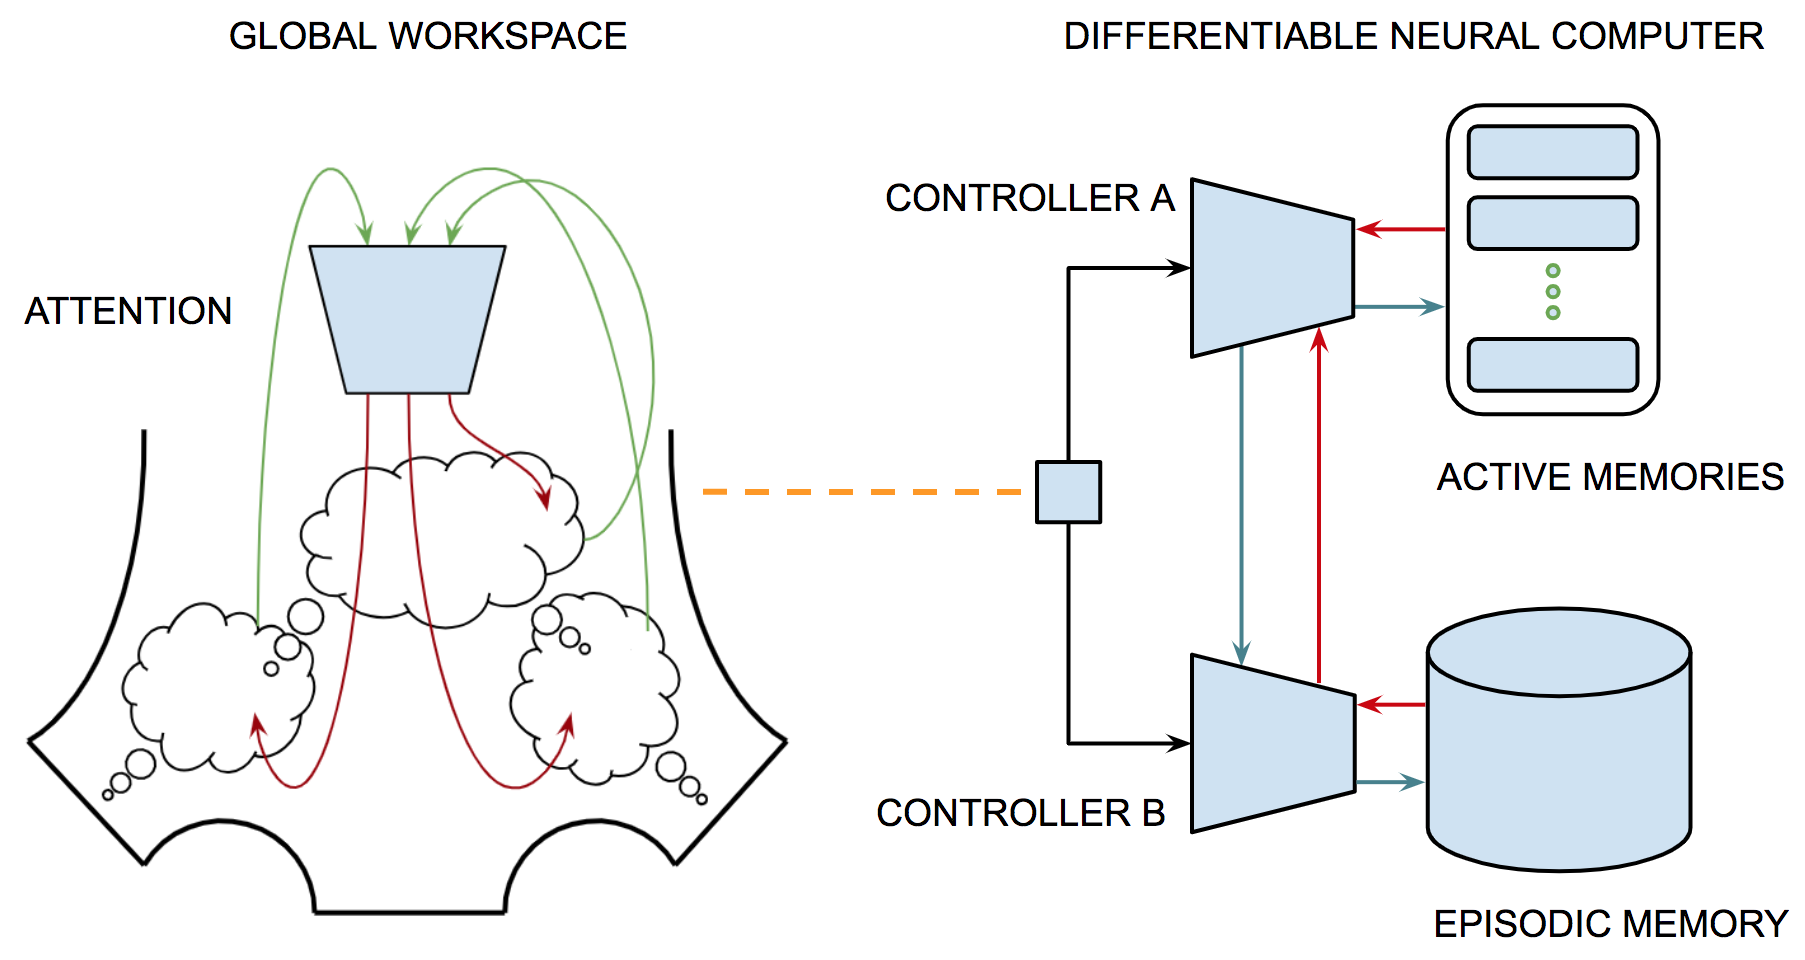
\includegraphics[width=590pt]{./figures/Global_Workspace_Episodic_Memory.png} % 1182 × 636 pixels
  \end{center}
%
  \caption{You can think of the episodic memory encoded in the hippocampus and entorhinal cortex as RAM and the actively maintained memories in the prefrontal cortex as the contents of registers in a conventional von Neumann architecture. Since the activated memories have different temporal characteristics and functional relationships with the contents of the global workspace, we implement them as two separate NTM memory systems each with its own special-purpose controller. Actively maintained information highlighted in the global workspace is used to generate keys for retrieving relevant memories that augment the highlighted activations. In the DNC paper~\cite{GravesetalNATURE-16} appearing in {\it{Nature}}, the authors point out that "an associative key that only partially matches the content of a memory location can still be used to attend strongly to that location [allowing] allowing the content of one address [to] effectively encode references to other addresses". The contents of memory consist of thought vectors that can be composed with other thought vectors to shape the global context for interpretation.}
%
  \hrule{}
%
\end{figure}

%%% %%%%%%%%%%%%%%%%%%%%%%%%%%%%%%%%%%%%%%%%%%%%%%%%%%%%%%%%%%%%%%%%%%%%%%%%%%%%

Figure~{\urlh{#fig_High_Level_Assistant_Architecture}{53}} combines the components that we've introduced so far in a single neural network architecture. The empty box on the far right includes both the language processing and dialogue management systems as well the networks that interface with FIDE and the other components involved in code synthesis. There are several classes of programming tasks that we might tackle in order to show off the apprentice, including commenting, extending, refactoring and repairing programs. We could focus on functional languages like Scheme or Haskell, strongly typed languages like Pascal and Java or domain specific languages like HTML or SQL. 

However, rather than emphasize any particular programming language or task, in the remainder of this appendix we focus on how one might represent structured programs consisting of one or more procedures in a distributed connectionist framework so as to exploit the advantages of this computational paradigm. We believe the highly-parallel, contextual, connectionist computations that dominate in human information processing will complement the primarily-serial, combinatorial, symbolic computations that characterize conventional information processing and will have a considerable positive impact on the development of practical automatic programming methods.

%%% %%%%%%%%%%%%%%%%%%%%%%%%%%%%%%%%%%%%%%%%%%%%%%%%%%%%%%%%%%%%%%%%%%%%%%%%%%%%

\setcounter{figure}{52}

%%% %%%%%%%%%%%%%%%%%%%%%%%%%%%%%%%%%%%%%%%%%%%%%%%%%%%%%%%%%%%%%%%%%%%%%%%%%%%%

%%% Figure~{\urlh{#fig_High_Level_Assistant_Architecture}{53}}
\rawhtml
<a name="fig_High_Level_Assistant_Architecture"></a>
\endrawhtml
\begin{figure}
%
  \hrule{}
%
  \begin{center} 
    % (* 1.375 (/ 1341 2.25)) = 595
    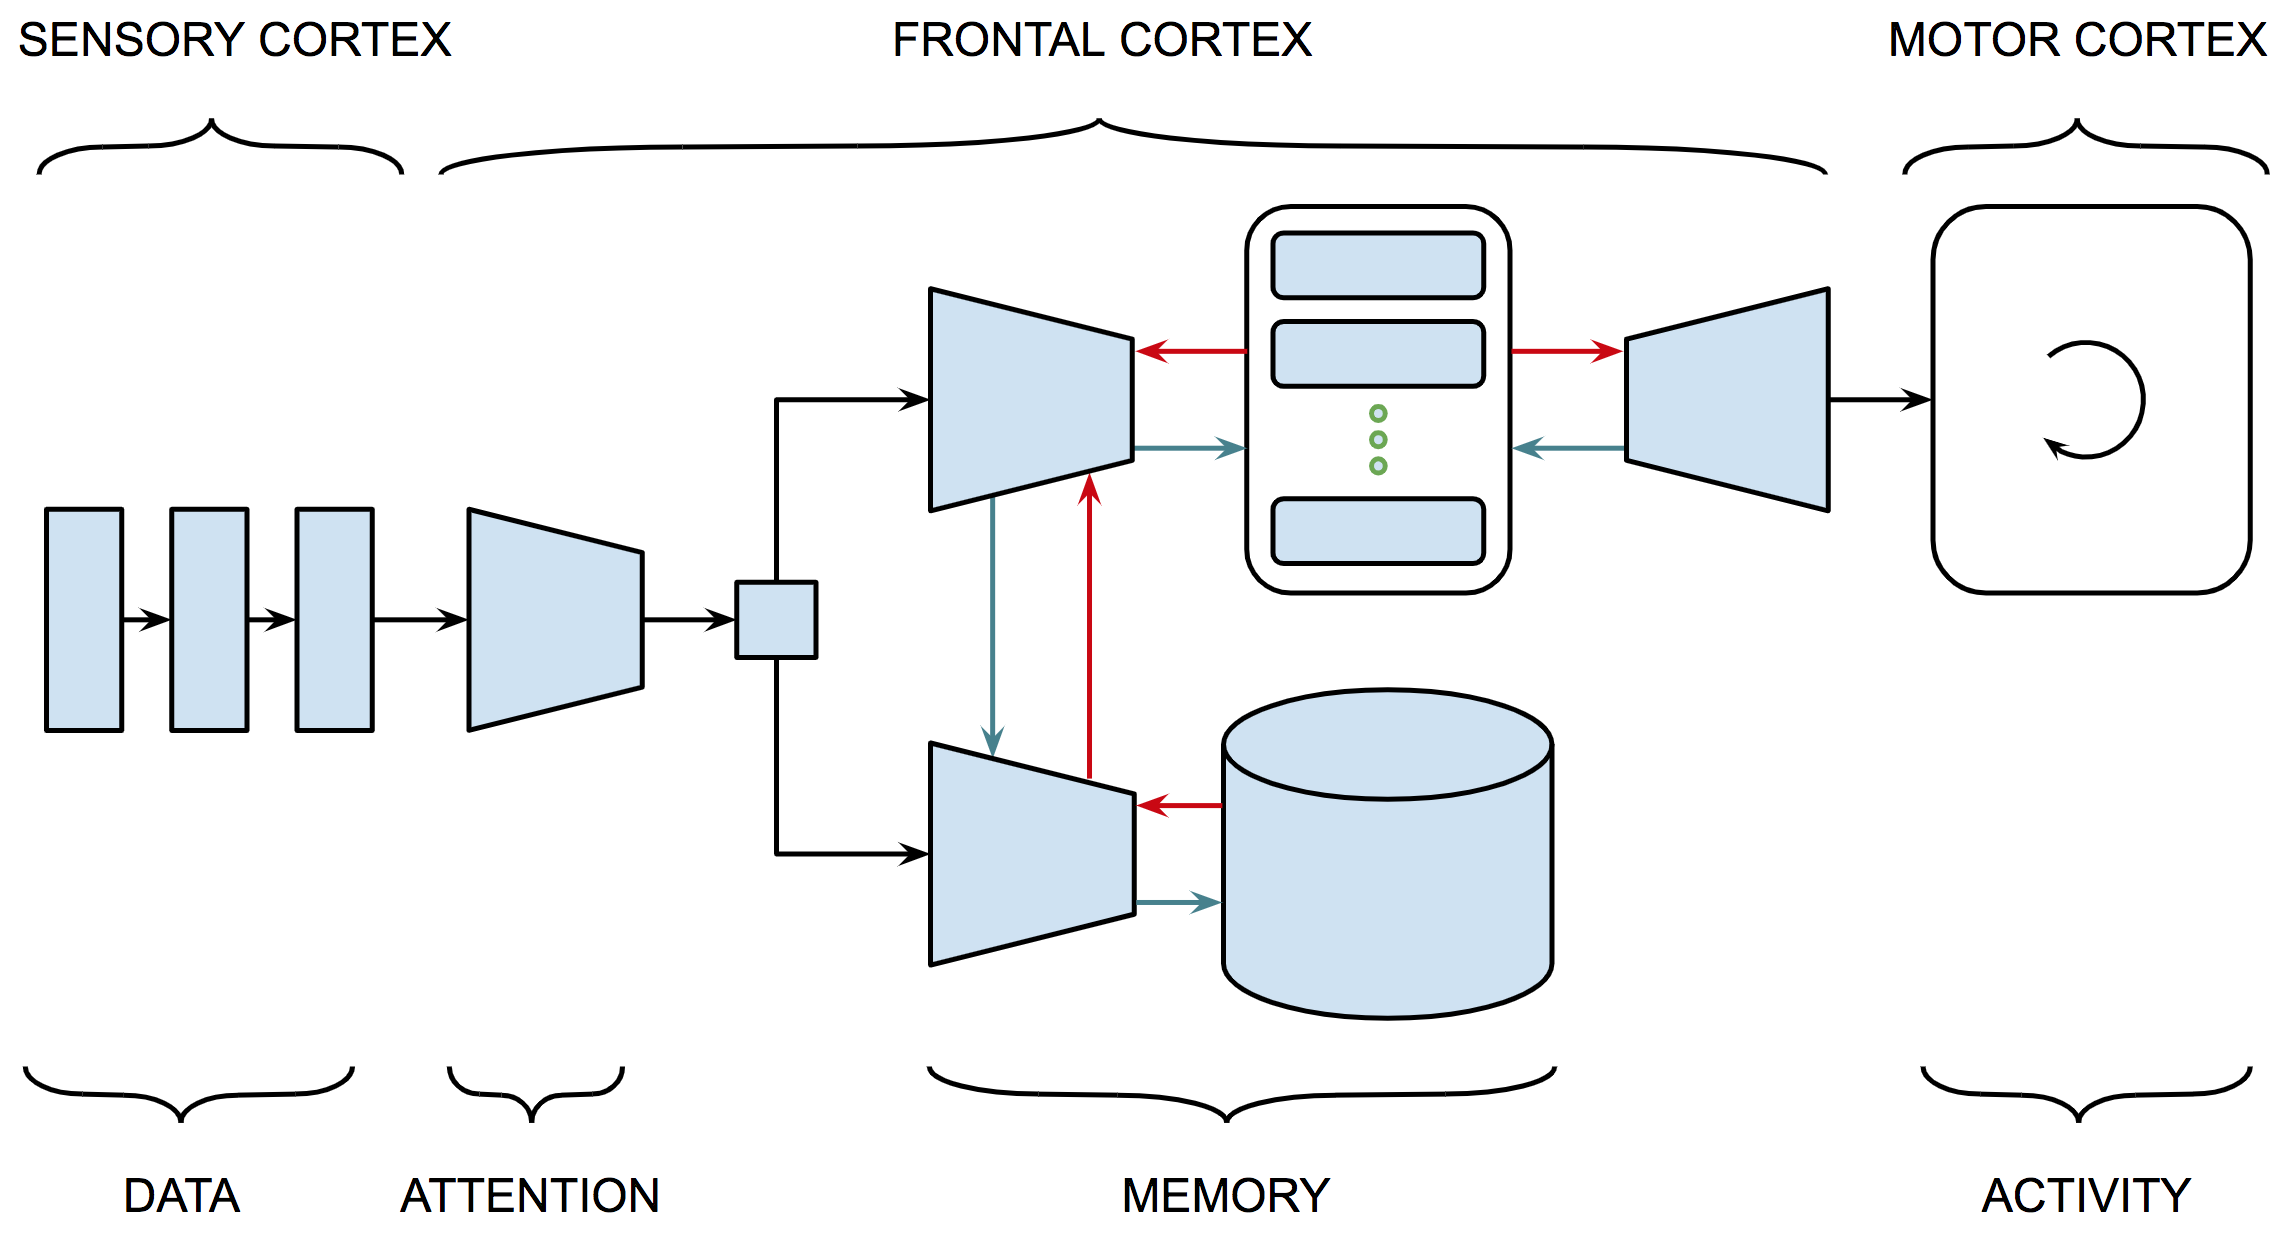
\includegraphics[width=595pt]{./figures/High_Level_Assistant_Architecture.png} % 1341 × 723 pixels  
  \end{center}
%
  \caption{This slide summarizes the architectural components introduced so far in a single model. Data in the form of text transcriptions of ongoing dialogue, source code and related documentation and output from the integrated development environment are the primary input to the system and are handled by relatively standard neural network models. The Q-network for the attentional RL system is realized as a multi-layer convolutional network. The two DNC controllers are straightforward variations on existing network models with a second controller responsible for maintaining a priority queue encodings of relevant past experience retrieved from episodic memory. The nondescript box labeled "motor cortex" serves as a placeholder for the neural networks responsible for managing dialogue and handling tasks related to programming and code synthesis.}
%
  \hrule{}
%
\end{figure}

%%% %%%%%%%%%%%%%%%%%%%%%%%%%%%%%%%%%%%%%%%%%%%%%%%%%%%%%%%%%%%%%%%%%%%%%%%%%%%%

The integrated development environment and its associated software engineering tools constitute an extension of the apprentice’s capabilities in much the same way that a piano or violin extends a musician or a prosthetic limb extends someone who has lost an arm or leg. The extension becomes an integral part of the person possessing it and over time their brain creates a topographic map that facilitates interacting with the extension\footnote{%
%
  In the mammalian brain, information pertaining to sensing and motor control is topographically mapped to reflect the intrinsic structure of that information required for interpretation. This was early recognized in the work of Hubel and Wiesel~\cite{HubelandWieselJoP-68,HubelandWieselJoP-62} on the striate cortex of the cat and macaque monkey and in the work of Wilder Penfield~\cite{PenfieldandBoldreyBRAIN-37} developing the idea of a cortical homunculus in the primary motor and somatosensory areas of the brain located between the parietal and frontal lobes of the primate cortex. Such maps have become associated with the theory of embodied cognition.}. 
 
As engineers designing the apprentice, part of our job is to create tools that enable the apprentice to learn its trade and eventually become an expert. Conventional IDE tools simplify the job of software engineers in designing software. The fully instrumented IDE (FIDE) that we engineer for the apprentice will be integrated into the apprentice’s cognitive architecture so that tasks like stepping a debugger or setting breakpoints are as easy for the apprentice as balancing parentheses and checking for spelling errors in a text editor is for us.

As a first step in simplifying the use of FIDE for coding, the apprentice is designed to manipulate programs as abstract syntax trees (AST) and easily move back and forth between the AST representation and the original source code in collaborating with the programmer. Both the apprentice and the programmer can modify or make references to text appearing in the FIDE window by pointing to items or highlighting regions of the source code. The text and AST versions of the programs represented in the FIDE are automatically synchronized so that the program under development is forced to adhere to certain syntactic invariants. 

%%% %%%%%%%%%%%%%%%%%%%%%%%%%%%%%%%%%%%%%%%%%%%%%%%%%%%%%%%%%%%%%%%%%%%%%%%%%%%%

\setcounter{figure}{53}

%%% %%%%%%%%%%%%%%%%%%%%%%%%%%%%%%%%%%%%%%%%%%%%%%%%%%%%%%%%%%%%%%%%%%%%%%%%%%%%

%%% Figure~{\urlh{#fig_Differentiable_Structured_Programs}{54}}
\rawhtml
<a name="fig_Differentiable_Structured_Programs"></a>
\endrawhtml
\begin{figure}
%
  \hrule{}
%
  \begin{center} 
    % (* 1.375 (/ 625 2.00)) = 325
    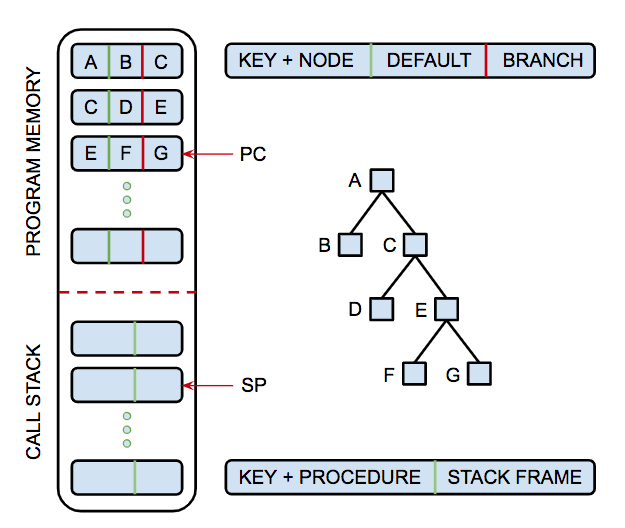
\includegraphics[width=325pt]{./figures/Differentiable_Structured_Programs.png} % 625 × 528 pixels
  \end{center}
%
  \caption{We use pointers to represent programs as abstract syntax trees and partition the NTM memory, as in a conventional computer, into program memory and a LIFO execution (call) stack to support recursion and reentrant procedure invocations, including call frames for return addresses, local variable values and related parameters. The NTM controller manages the program counter and LIFO call stack to simulate the execution of programs stored in program memory. Program statements are represented as embedding vectors and the system learns to evaluate these representations in order to generate intermediate results that are also embeddings. It is a simple matter to execute the corresponding code in the FIDE and incorporate any of the results as features in embeddings.}
%
  \hrule{}
%
\end{figure}

%%% %%%%%%%%%%%%%%%%%%%%%%%%%%%%%%%%%%%%%%%%%%%%%%%%%%%%%%%%%%%%%%%%%%%%%%%%%%%%

To support this hypothesis, we are developing distributed representations for programs that enable the apprentice to efficiently search for solutions to programming problems by allowing the apprentice to easily move back and forth between the two paradigms, exploiting both conventional approaches to program synthesis and recent work on machine learning and inference in artificial neural networks. Neural Turing Machines coupled with reinforcement learning are capable of learning simple programs. We are interested in representing structured programs expressed in modern programming languages. Our approach is to alter the NTM controller and impose additional structure on the NTM memory designed to support procedural abstraction. 

What could we do with such a representation? It is important to understand why we don’t work with some intermediate representation like bytecodes. By working in the target programming language, we can take advantage of both the abstractions afforded by the language and the expert knowledge of the programmer about how to exploit those abstractions. The apprentice is bootstrapped with several statistical language models: one trained on a natural language corpus and the other on a large code repository. Using these resources and the means of representing and manipulating program embeddings, we intend to train the apprentice to predict the next expression in a partially constructed program by using a variant of imagination-based planning~\cite{PascanuetalCoRR-17}. As another example, we will attempt to leverage NLP methods to generate proposals for substituting one program fragment for another as the basis for code completion. 

%%% %%%%%%%%%%%%%%%%%%%%%%%%%%%%%%%%%%%%%%%%%%%%%%%%%%%%%%%%%%%%%%%%%%%%%%%%%%%%

\setcounter{figure}{54}

%%% %%%%%%%%%%%%%%%%%%%%%%%%%%%%%%%%%%%%%%%%%%%%%%%%%%%%%%%%%%%%%%%%%%%%%%%%%%%%

%%% Figure~{\urlh{#fig_Differentiable_Program_Emulation}{55}}
\rawhtml
<a name="fig_Differentiable_Program_Emulation"></a>
\endrawhtml
\begin{figure}
%
  \hrule{}
%
  \begin{center} 
    % (* 1.375 (/ 918 2.75)) = 325
    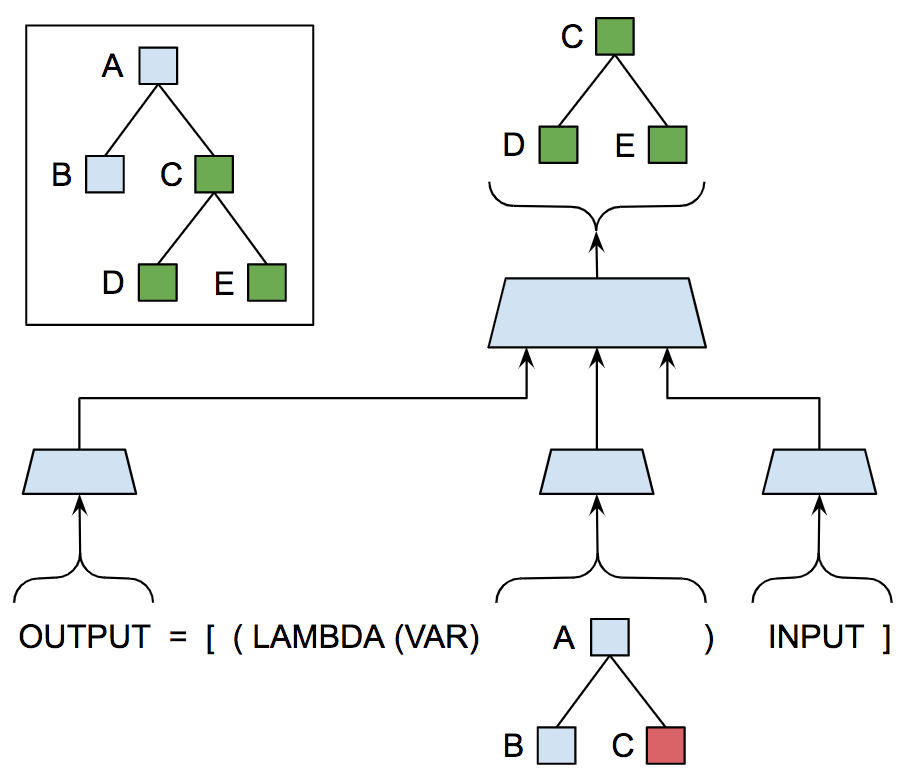
\includegraphics[width=325pt]{./figures/Differentiable_Program_Emulation.png} % 918 × 781 pixels
  \end{center}
%
  \caption{This slide illustrates how we make use of input / output pairs as program invariants to narrow search for the next statement in the evolving target program. At any given moment the call stack contains the trace of a single conditioned path through the developing program. A single path is unlikely to provide sufficient information to account for the constraints implicit in all of the sample input / output pairs and so we intend to use a limited lookahead planning system to sample multiple execution traces in order to inform the prediction of the next program statement. 
%
These so-called imagination-augmented agents implement a novel architecture for reinforcement learning that balances exploration and exploitation using imperfect models to generate trajectories from some initial state using actions sampled from a rollout policy~\cite{PascanuetalCoRR-17,WeberetalCoRR-17,HamricketalCoRR-17,GuezetalCoRR-18}. These trajectories are then combined and fed to an output policy along with the action proposed by a model-free policy to make better decisions. There are related reinforcement learning architectures that perform Monte Carlo Markov chain search to apply and collect the constraints from multiple input / output pairs.}
%
  \hrule{}
%
\end{figure}

%%% %%%%%%%%%%%%%%%%%%%%%%%%%%%%%%%%%%%%%%%%%%%%%%%%%%%%%%%%%%%%%%%%%%%%%%%%%%%%

The Differentiable Neural Program (DNP) representation and associated NTM controller for managing the call stack and single-stepping through such programs allow us to exploit the advantages of distributed vector representations to predict the next statement in a program under construction. This model makes it easy to take advantage of supplied natural language descriptions and example input / output pairs plus incorporate semantic information in the form of execution traces generated by utilizing the FIDE to evaluate each statement and encoding information about local variables on the stack. 

%%% %%%%%%%%%%%%%%%%%%%%%%%%%%%%%%%%%%%%%%%%%%%%%%%%%%%%%%%%%%%%%%%%%%%%%%%%%%%%
